\chapter{Perancangan}
\label{chap:perancangan}
Pada bab ini akan dijelaskan perancangan perangkat lunak yang dibuat pada penelitian ini. Perancangan terdiri dari masukan perangkat lunak dan diagram aktivitas. 

\section{Masukan Perangkat Lunak}
\label{sec:inputConfig} 
Perangkat lunak perekaman kehadiran daring otomatis membutuhkan 1 file sebagai masukan, yaitu \textit{file} .ini (\textit{file} konfigurasi). Pada \textit{file} .ini, nomor baris sebagai \textit{keys} dan \textit{string} berupa kata yang merupakan fungsi dari Selenium WebDriver dan elemen yang diambil untuk melakukan perekaman kehadiran daring otomatis sebagai \textit{values}. 

\subsection{Spesifikasi Masukan Perangkat Lunak}
\textit{File} konfigurasi terdiri dari \textit{section}, \textit{key}, dan \textit{value}. \textit{Section} ini merupakan judul dari \textit{file} konfigurasi. \textit{Key} akan berisi angka secara terurut dan dimulai dari angka satu hingga seterusnya, fungsi angka ini sebagai penanda urutan langkah-langkah yang nantinya akan dijalankan secara terurut oleh perangkat lunak. \textit{Value} merupakan isi dari \textit{key}, \textit{value} terdiri dari kata kunci untuk perangkat lunak menjalankan perintah dan elemen yang telah diambil dari situs web untuk melakukan otomatisasi, berikut ini adalah penjelasan kata kunci pada \textit{value}:
\begin{itemize}
	\item Kata \textit{open} merupakan kata kunci bagi perangkat lunak untuk membuka situs web yang ingin dituju. 
	\item Kata \textit{click} merupakan kata kunci bagi perangkat lunak untuk menekan suatu tombol secara otomatis sesuai dengan elemen yang telah diambil pada situs web yang telah dibuka.
	\item Kata \textit{sendkeys} merupakan kata kunci bagi perangkat lunak untuk mengetik atau memasukan suatu nilai dalam bentuk teks maupun angka secara otomatis pada suatu elemen yang telah diambil.
	\item Kata \textit{or} merupakan kata kunci bagi perangkat lunak untuk melihat dua kemungkinan yang terjadi dan menekan tombol secara otomatis pada satu elemen yang telah diambil atau dua elemen yang telah diambil secara bertahap.  
	\item Kata \textit{quit} merupakan kata kunci bagi perangkat lunak untuk menutup browser.
\end{itemize}

\subsection{Kontrusksi Masukan Perangkat Lunak}
Perancangan untuk penulisan \textit{file} .ini 

Berikut ini adalah contoh serta penjelasan \textit{file} .ini dapat dilihat pada Listing \ref{kode:4:conf}.
\begin{lstlisting}[caption=Contoh \textit{file} .ini untuk Masukan Perangkat Lunak Perekaman Kehadiran Daring Otomatis, label=kode:4:conf]
	[database_config]
	1 = open https://studentportal.unpar.ac.id
	2 = click #login-button
	3 = sendkeys #username 2017730035@student.unpar.ac.id 
	4 = quit
\end{lstlisting}
Berikut ini penjelasan dari isi dari contoh \textit{file} .ini:
\begin{itemize}
	\item Baris pertama berisi nama \textit{section} untuk isi \textit{file} .ini.
	\item \textit{keys} pada \textit{file} .ini ini pasti berupa angka yang terurut agar perangkat lunak dapat menjalankannya secara terurut.
	\item Terdapat 4 fungsi kata dari Selenium WebDriver, yaitu \textit{open}, \textit{click}, \textit{sendkeys}, dan \textit{quit}.
	\item \textit{Keys} 1 pasti diisi oleh fungsi \textit{open}, lalu diisi situs web (\url{https://studentportal.unpar.ac.id}), karena langkah pertama setelah berhasil membuka browser adalah menuju pada situs web yang akan diotomatisasi.
	\item \textit{Keys} 2 memiliki fungsi \textit{click} untuk menekan tombol secara otomatis dan diisi elemen ``\#login-button'' yang diambil berdasarkan CSS Selector.
	\item \textit{Keys} 3 memiliki fungsi \textit{sendkeys} untuk memasukan suatu nilai ke dalam elemen yang dipilih, yaitu elemen ``\#username'' dan isinya adalah ``2017730035@student.unpar.ac.id''.
	\item \textit{Keys} 4 memiliki fungsi \textit{quit} untuk menutup browsernya.
\end{itemize}
Elemen yang dipakai dalam \textit{file} .ini ini diambil dengan cara melakukan \textit{inspect element} pada web yang ingin dilakukan otomatisasi. Pada Gambar \ref{fig:inspect} adalah cara yang dilakukan untuk mendapat elemen yang ingin digunakan untuk melakukan otomatisasi. Untuk mendapatkan elemen tersebut, perlu melakukan klik kanan pada bagian elemen yang ingin diambil, lalu pilih ``inspect''. Setelah melakukan ``inspect'' maka akan muncul dokumen HTML yang dapat dilihat pada bagian kanan Gambar \ref{fig:inspect}, sehingga dapat melakukan pengambilan elemen yang diperlukan.
\begin{figure}[H]
	\centering
	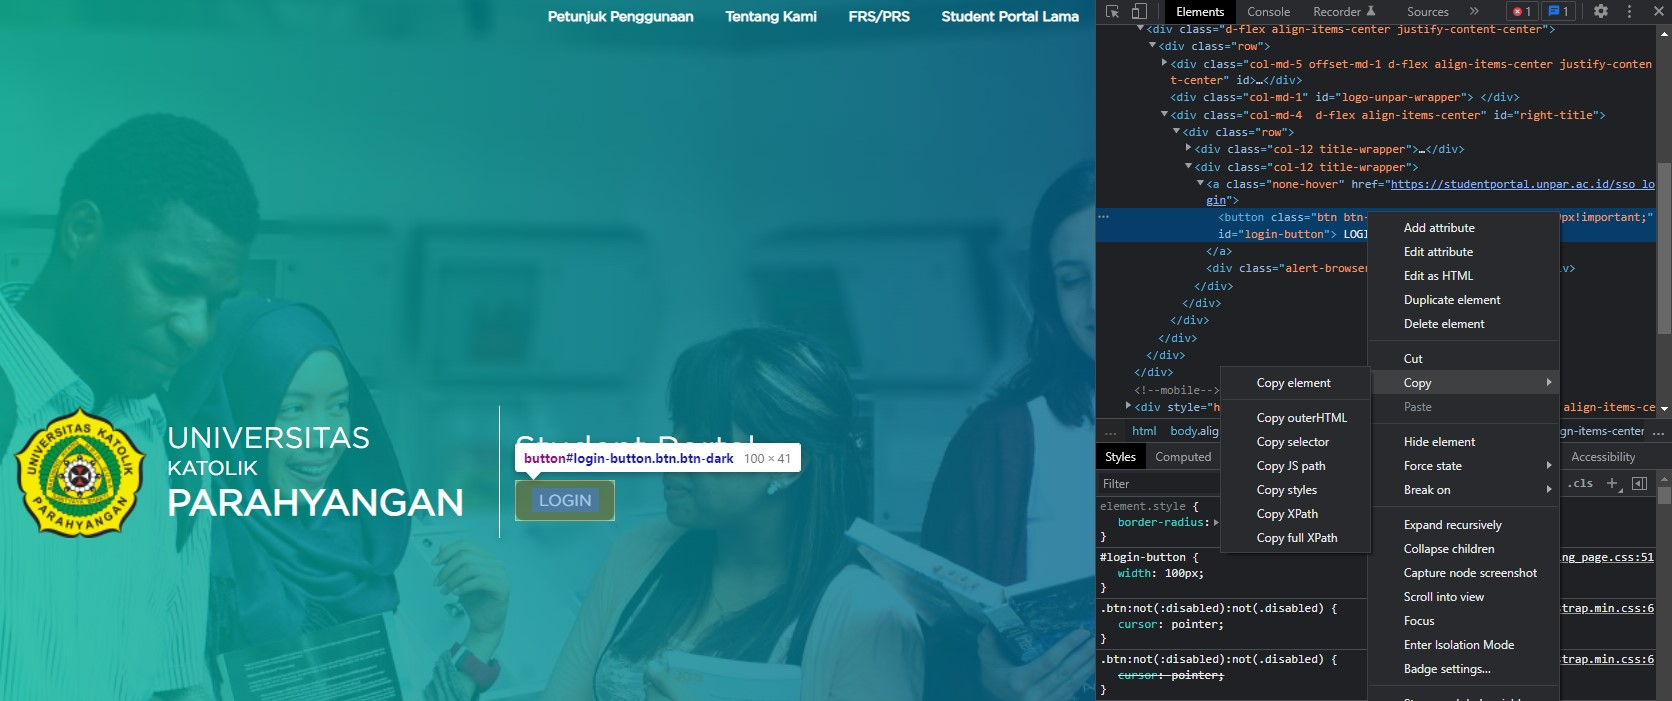
\includegraphics[scale=0.3]{Gambar/elemen.jpg}
	\caption{Tampilan Melakukan \textit{Inspect Element}} 
	\label{fig:inspect}
\end{figure}	

\section{Diagram Aktivitas}
\label{sec:diagramAktivitas}
Perangkat lunak perekaman absen daring otomatis adalah perangkat lunak yang digunakan untuk melakukan absensi secara otomatis bagi mahasiswa UNPAR. Perangkat lunak ini menggunakan Selenium WebDriver sebagai \textit{tools} yang berguna untuk melakukan otomatisasi pada browser web. Perangkat lunak ini juga membutuhkan masukan dari sebuah file konfigurasi untuk menjalankannya.
Diagram Aktivitas untuk \textit{setup} menjalankan program dan menyiapkan file konfigurasi dapat dilihat Gambar \ref{fig:ActivitySetup}. Berikut ini adalah penjelasan langkah-langkah pada diagram aktivitas:
\begin{enumerate}
	\item Pengguna melakukan \textit{install} python, karena program perekaman absen daring otomatis menggunakan bahasa pemrograman python.
	\item Pengguna melakukan \textit{install} selenium, karena untuk melakukan perekaman absen daring secara otomatis menggunakan selenium.
	\item Pengguna melakukan \textit{install} chrome driver, karena menggunakan browser Google Chrome untuk melakukan perekaman absen daring otomatis.
	\item Pengguna membuka file konfigurasi dan mengubah email serta password sesuai milik pengguna agar dapat digunakan sebagai masukan pada perangkat lunak untuk melakukan perekaman absen daring otomatis.
	asdasfgadsgasdf
	\item Pengguna menyimpan hasil perubahan yang telah dilakukan pada file konfigurasi. BELUM SELESAI !!!!!!!!!!!!!!!!!
\end{enumerate}
\begin{figure}[H]
	\centering
	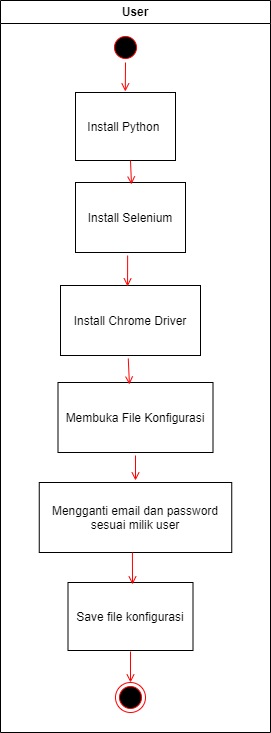
\includegraphics[scale=0.4]{Gambar/ActivitySetup.png}
	\caption{Diagram Aktivitas untuk \textit{Setup} Menjalankan Program} 
	\label{fig:ActivitySetup}
\end{figure}
Diagram Aktivitas untuk perangkat lunak perekaman kehadiran daring otomatis dapat dilihat pada Gambar \ref{fig:ActivityAplikasi}. Berikut ini adalah penjelasan langkah-langkah pada diagram aktivitas:
\begin{enumerate}
	\item Pengguna menjalankan langsung programnya.
	\item Perangkat lunak akan membuka browser Google Chrome saat pertama kali program dijalankan.
	\item Perangkat lunak menerima masukan dari file konfigurasi yang telah di-\textit{setup} oleh pengguna.
	\item Perangkat lunak akan menjalankan perintah sesuai masukan file konfigurasi secara baris perbaris.
	\item Perangkat lunak akan melakukan \textit{looping} jika masukkan dari file konfigurasi berisi kata ``\textit{open}'' maka perangkat lunak akan membuka situs web yang dituju.
	\item 
	\item
\end{enumerate}
\begin{figure}[H]
	\centering
	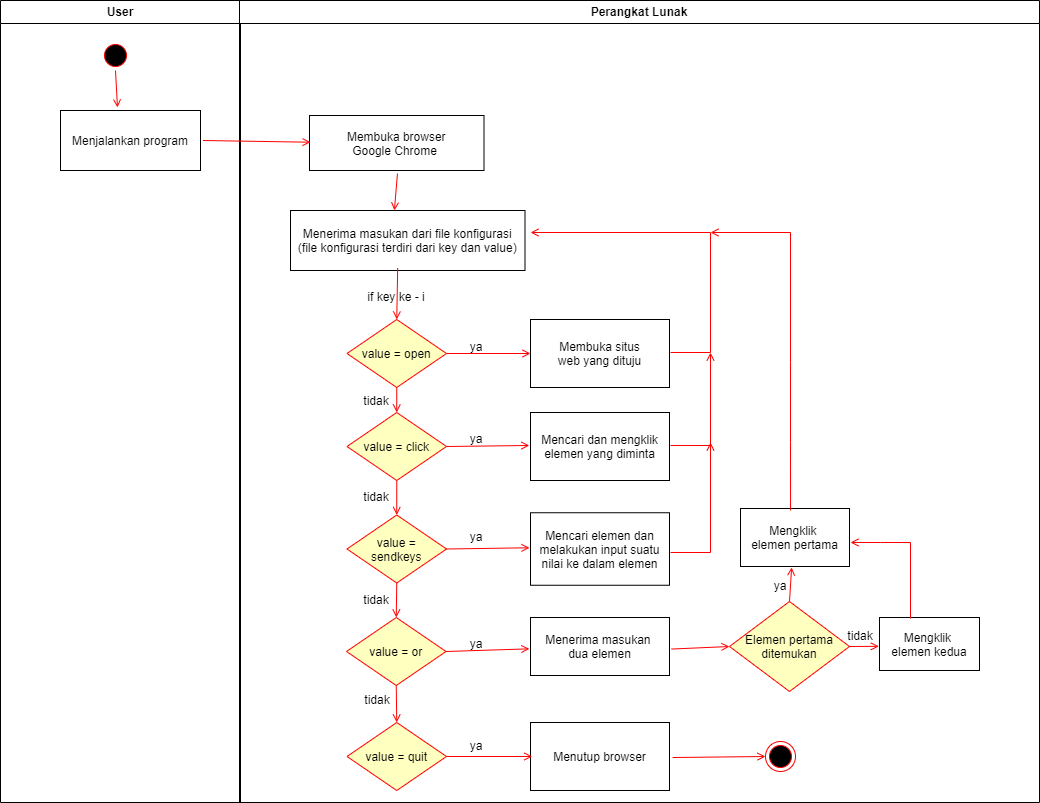
\includegraphics[scale=0.4]{Gambar/ActivityAplikasi.png}
	\caption{Diagram Aktivitas Perangkat Lunak Absen Daring Otomatis} 
	\label{fig:ActivityAplikasi}
\end{figure}

